\section{Evaluation}

We conducted three user studies, iteratively refining the \chameleon{} UI and evaluating several research questions as per Fig.~\ref{fig:timeline}. 



\begin{figure}
    \centering
    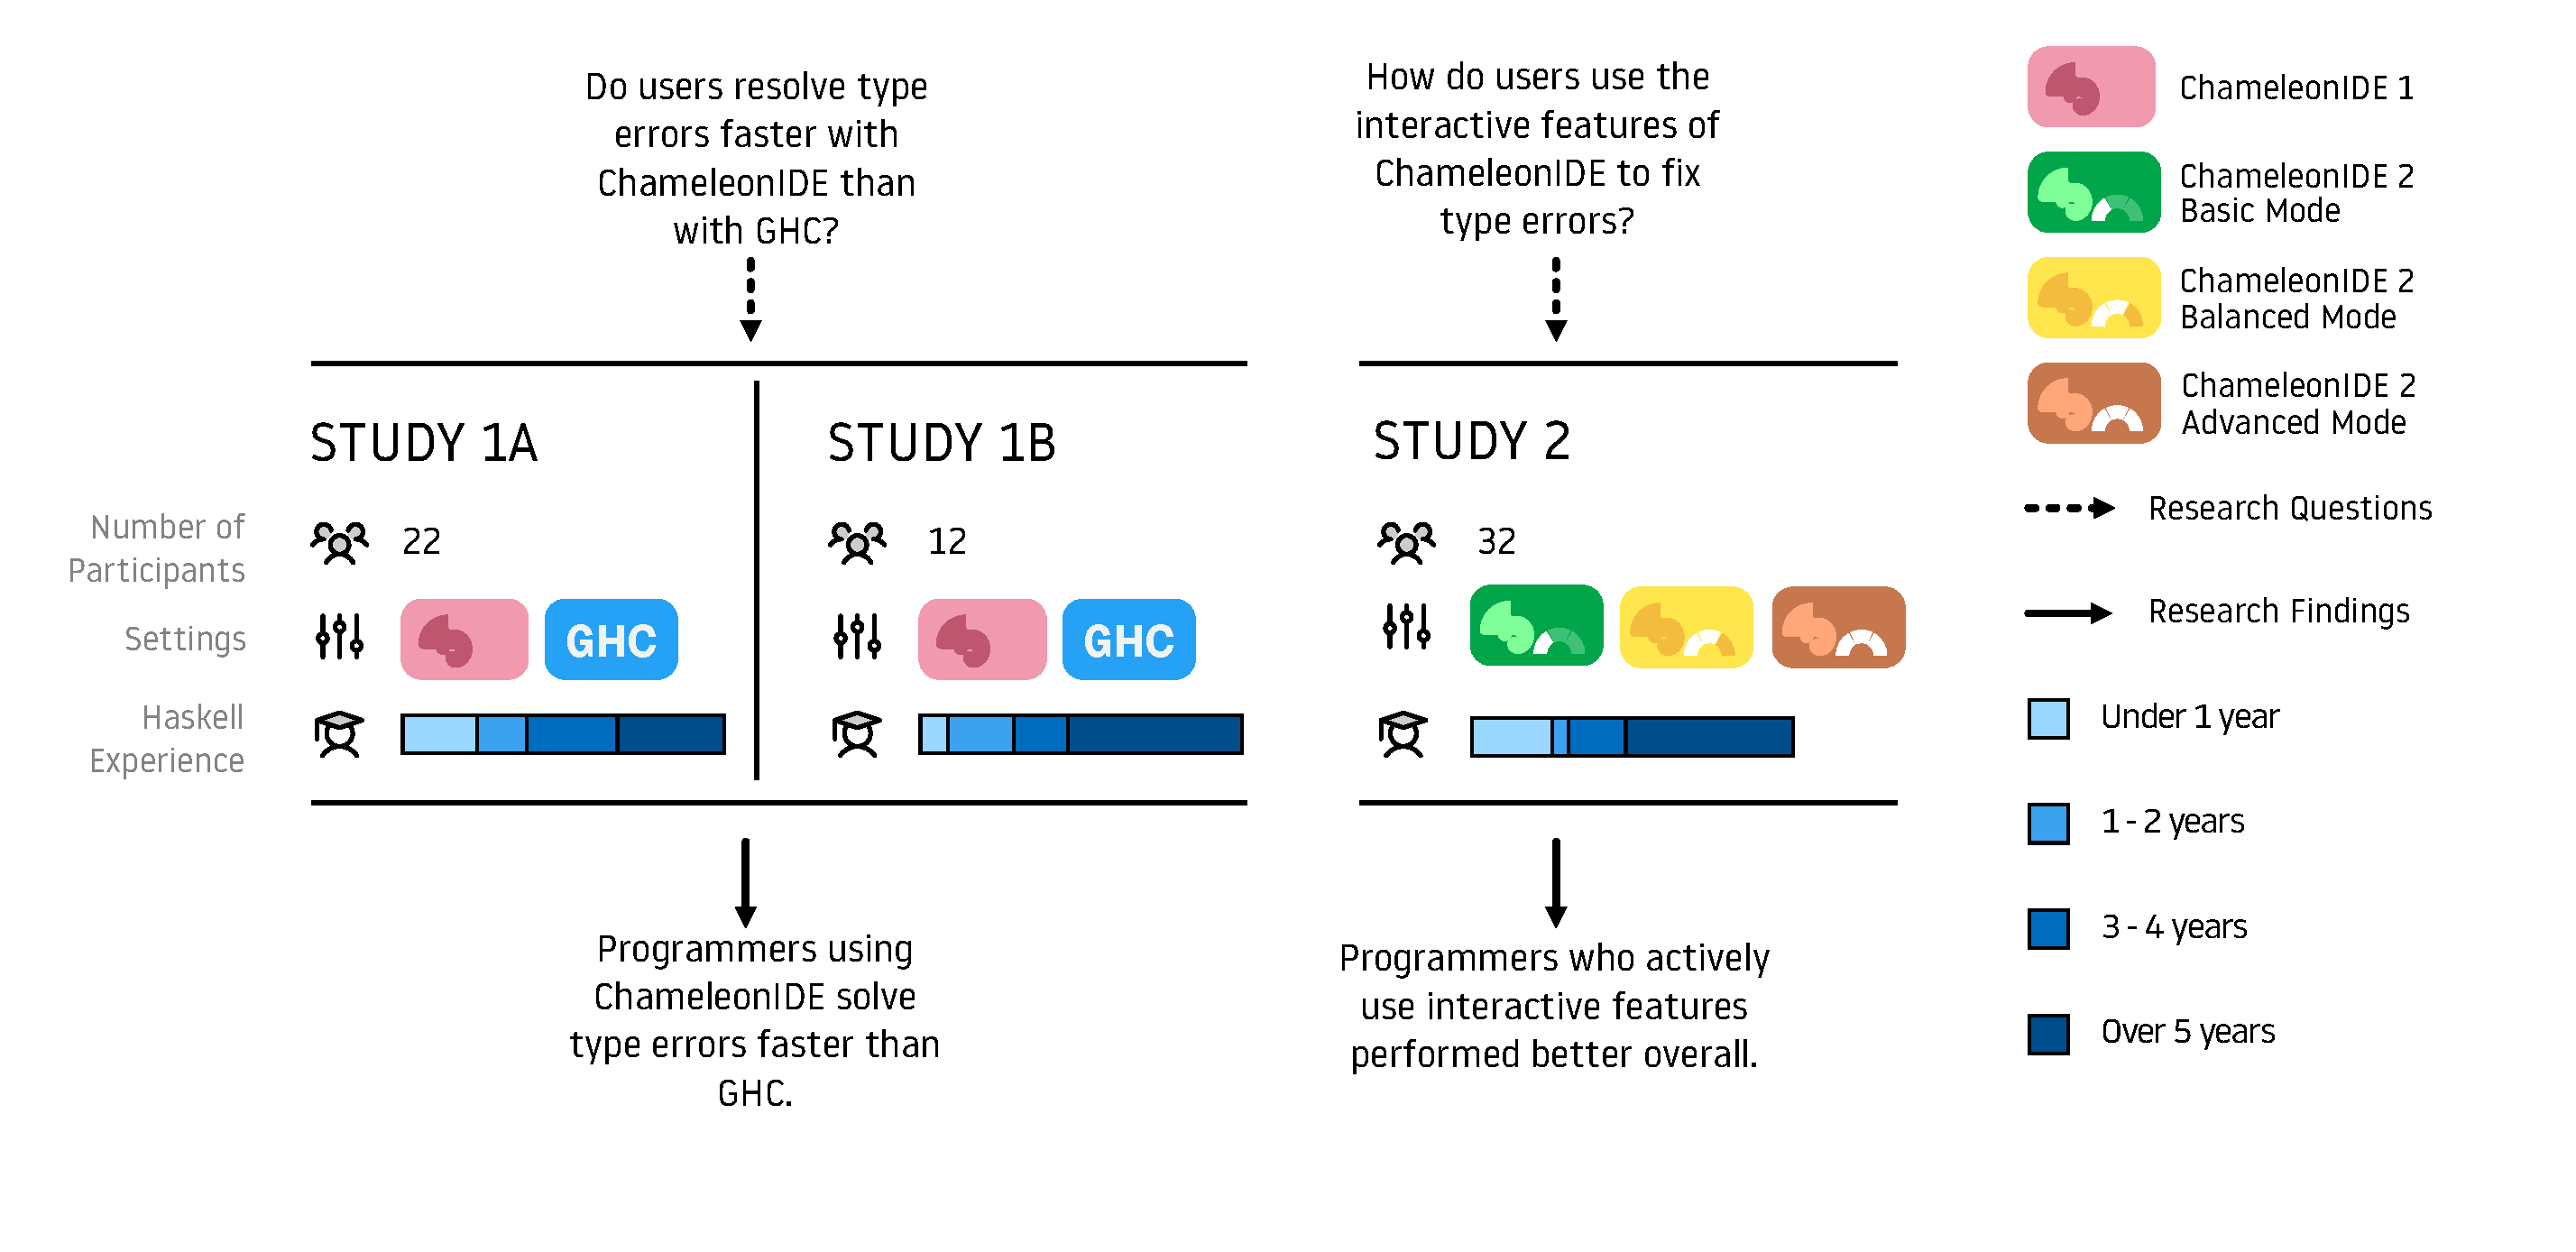
\includegraphics[width=\columnwidth,trim=30mm 35mm 35mm 5mm]{images/timeline.pdf}
    \caption[The timeline of \chameleon{}  evaluation]{The timeline of \chameleon{}  evaluation.}
    \label{fig:timeline}
\end{figure}

\subsection{Experiment Design}
\subsubsection*{\textbf{Recruitment}}

Participants were recruited via the Reddit \textit{r/haskell} and \textit{r/programminglanguages} communities. 
%Recruiting from social media allowed us to access a more diverse demographic that better represent the true population of Haskell programmers. 
Participation is fully anonymized; detailed ethical implications of these experiments are reviewed and approved by the IRB of the authors' institution.


\subsubsection*{\textbf{Experiment setting}}
Experiments were conducted online and unsupervised. 
%Participants took the study online via a web browser and at the physical venue of their choosing. 
All user studies use a web-based debugging environment developed by the authors. 
%Conducting the studies online helped us avoid variation when performing tasks in unfamiliar places and using different setups. 


\subsubsection*{\textbf{Training and group assignment}}
After consent, participants received interactive training on the tool interface and interactive features. Participants were also shown a cheat sheet summarizing the key functionality of the interface, and had access to the cheat sheet at all times during the study. Participants were given 4 trial runs (2 for each setting) before the data collection started. 
All the studies used a within-subject design to evaluate the effectiveness of different tools or feature sets while counterbalancing the difference in programming proficiency between participants. In each study, participants were required to complete a series of programming tasks (8 for studies 1a and 1b, 9 for study 2). At each task, a participant receives a single Haskell file that contains one or more type errors. They were then asked to correct the code with the help of the given tool.


\subsubsection*{\textbf{Data Collection}}
Time is measured from the start of each task to the first time the program is successfully type-checked and also passes all the functional tests. Participants are able to skip a task if they are stuck. 
% The data is automatically recorded by the online debugging environment. To not introduce a barrier to completing the study, every task can be skipped if the participant made three failed attempts or is stuck for over 1 minute on the task.
After completing all tasks, participants are prompted to complete a debriefing survey. The survey questions include their Haskell experience and feedback on the tools.

We used a browser session recording tool~\cite{OpenReplay2022-nw} to record the study sessions. This allows us to identify usability issues in the study and to recognize general patterns. 
%The reason we found this format inferior is that the recording technology does not provide a high enough sampling rate for us to be confidently used for rigorous analysis.
%One use of the session recording is for outlier trimming.  We identify participants who left the computer for an extended period of time. We first ran a statistical analysis to identify the long gap (2 standard deviations) between actions using program logs for each participant. Then, we manually checked with the session recording to verify there was actually no user input (mouse movement, scrolling). 

\subsection{\chameleon{} Human Studies}

\subsubsection{\textbf{\chameleon{} 1}}  
An earlier version of the UI than that depicted in Figs.~(2-13), it featured the type inference engine that recovers most concrete types after type errors occur and a minimal set of debugging features. Key features in \chameleon{} 1 include showing two (or more) alternative types, showing all possible error locations, dividing possible error locations into groups based on alternative types, and concrete type restoration. In short, \chameleon{} 1 is equivalent to \chameleon{} 2 set to basic mode. 

% \begin{figure}[h]
%     \centering
%     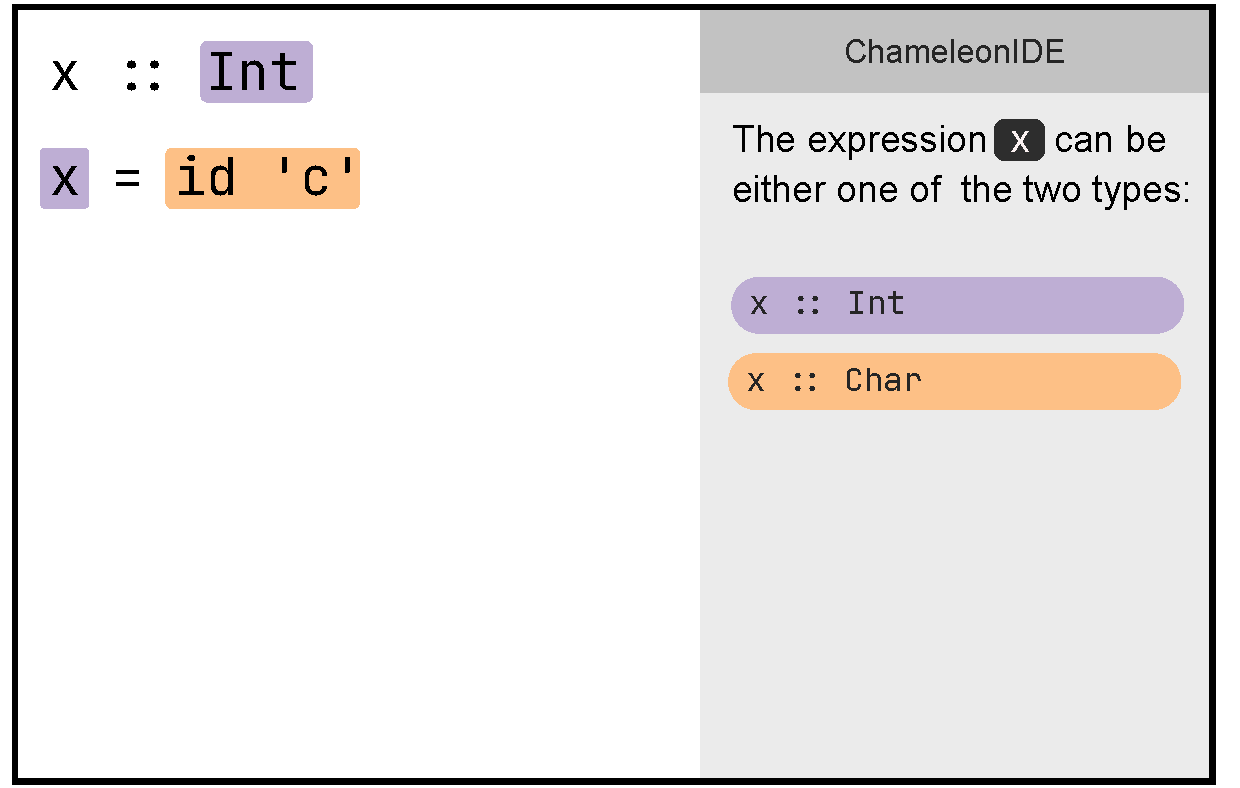
\includegraphics[width=\linewidth]{images/chameleon-v1.pdf}
%     \caption{
%         \chameleon{} 1
%         }
%     \label{fig:chameleon-v1}
% \end{figure}

Two  studies (1a \& 1b) were conducted to compare the effectiveness of solving type errors using \chameleon{} 1 and GHC compiler error messages. We choose GHC compiler error messages as the baseline because it is the canonical tool for working with type errors in Haskell.
%Although high-level tools like Haskell Language Server exist, they generally relay the GHC error messages verbatim. 
% The procedure of these studies is shown in figure \ref{fig:procedure-1}.


Eight tasks were given in both studies. In study 1a, the tasks were taken from the exercises of the Haskell programming class in the authors' institute. In the second study, the tasks are sourced from the top 20 Haskell topics on GitHub~\cite{Github2022-nm}. The authors then manually added type errors into the program. In both studies, the type errors include simple mismatch, confusing syntax, missing instance, precedence and fixation, infinite types, and confusing list versus element. These categories follow the common type errors in Tirronen's study \cite{Tirronen2015-nr}. 

Studies (1a \& 1b) address the research question:

\noindent\textbf{RQ1.} \textit{Do programmers solve type errors faster with \chameleon{} than GHC compiler error messages?}


% \begin{figure}[h]
%     \centering
%     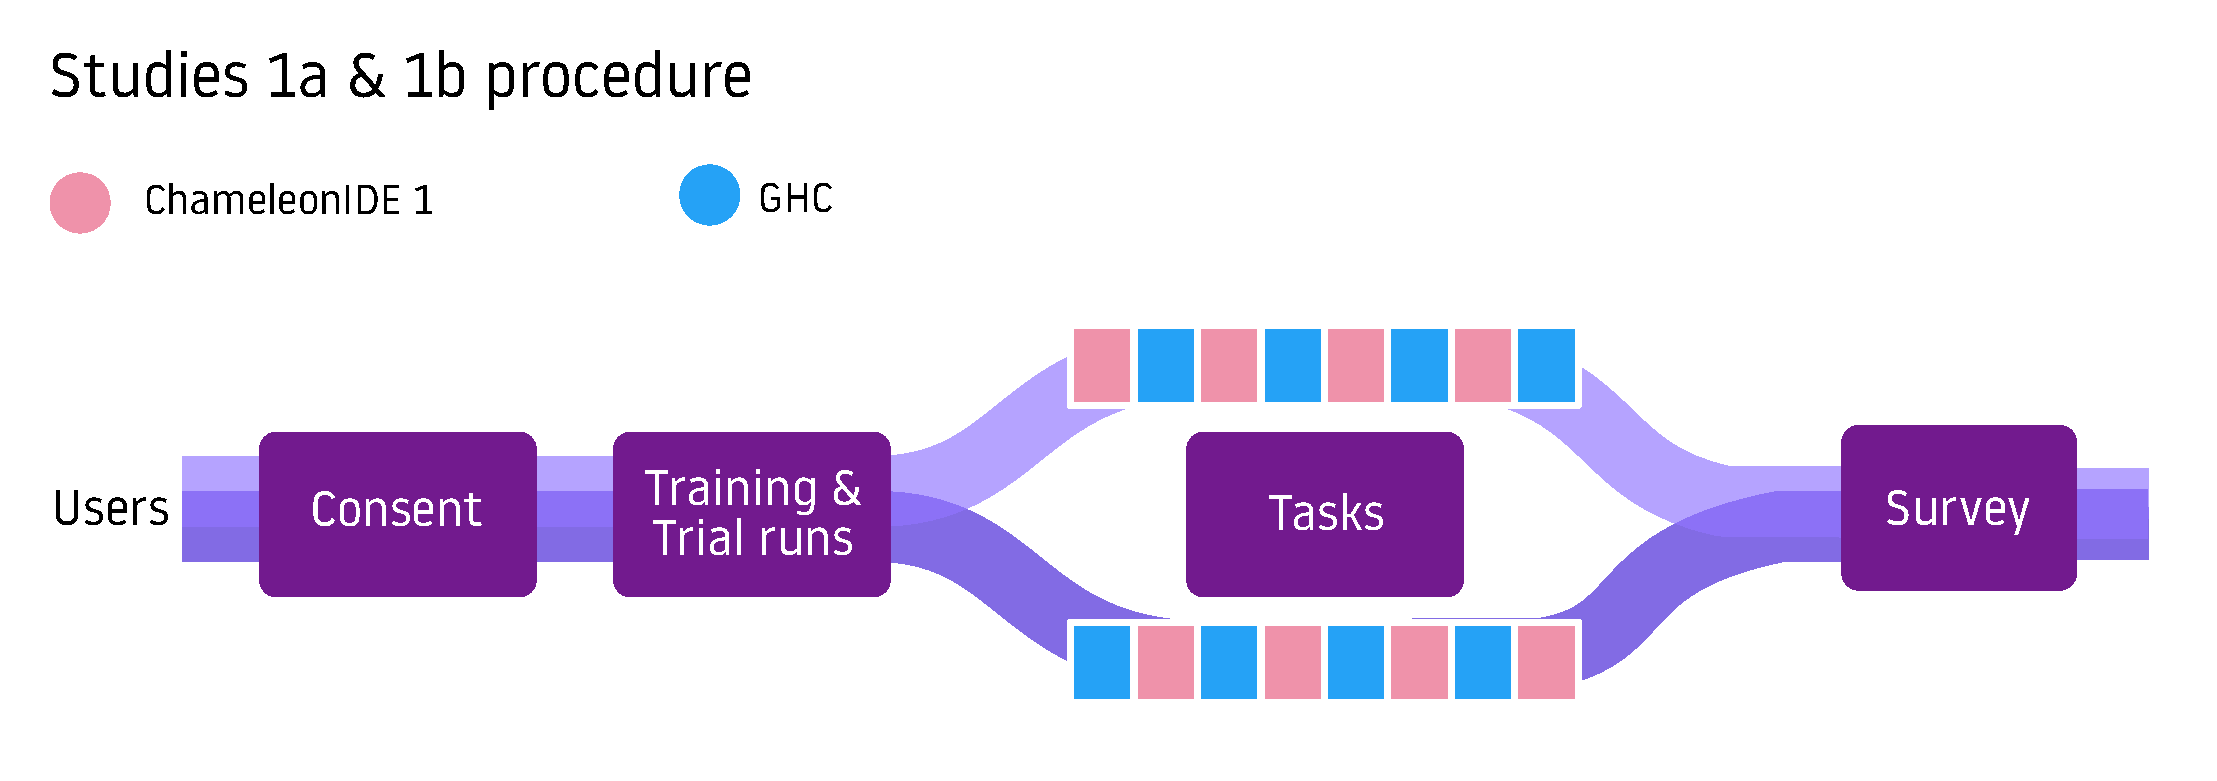
\includegraphics[width=\linewidth]{images/procedure-1.pdf}
%     \caption{\todo{Does this figure really help at all?}}
%     \label{fig:procedure-1}
% \end{figure}

% The study investigates the effectiveness of \chameleon{} compared to the GHC compiler error messages. We chose GHC compiler error messages as it is the canonical tool for debugging type errors in Haskell. Although high-level tools like Haskell Language Server exist, they relay the GHC error message verbatim for type errors. Participants are asked to complete 8 tasks. The tool participants used during each task alternated between \chameleon{} and GHC. Task programs were sourced from HaskellWiki \cite{haskellwiki}. The author manually added type errors. The errors cover a range of common Haskell type errors, including abstract data types, wrong arity, control expressions (if and case), infinite types, and tuples. The lines of code (LoC) range from 7 to 17 (mean = 11, median=10.5).


% In total 39 participants finished the study. Among them, 12 participants have over five years of Haskell experience, and 5 participants have three or four years of Haskell experience. And 8 participants have one or two years of experience, and 5 participants used Haskell for under a year. The rest left the question unanswered.

\begin{figure}
    \centering
    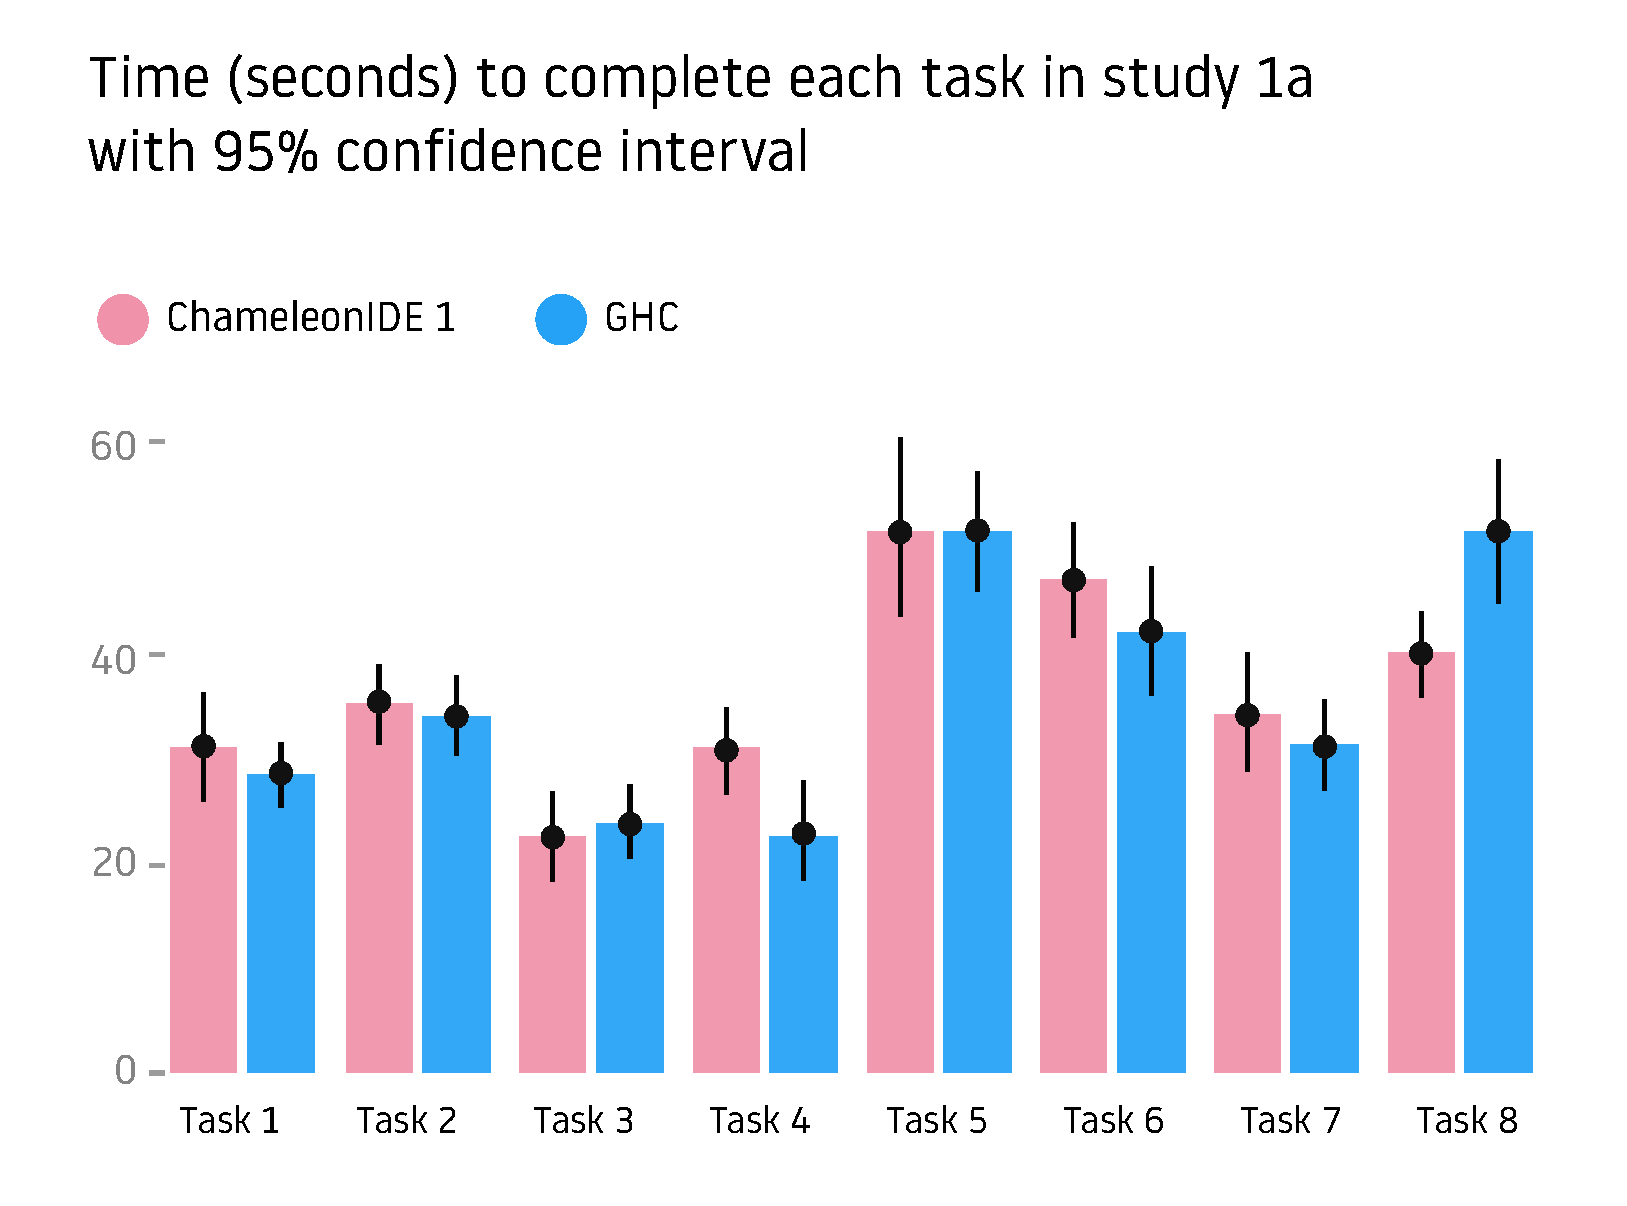
\includegraphics[width=0.8\linewidth,trim=15mm 12mm 15mm 35mm,clip]{images/user-study-1a.pdf}
    \caption{Study 1a task completion time (secs.) with 95\% confidence interval.}
    \label{fig:analysis-1a}
\end{figure}


\begin{figure}
    \centering
    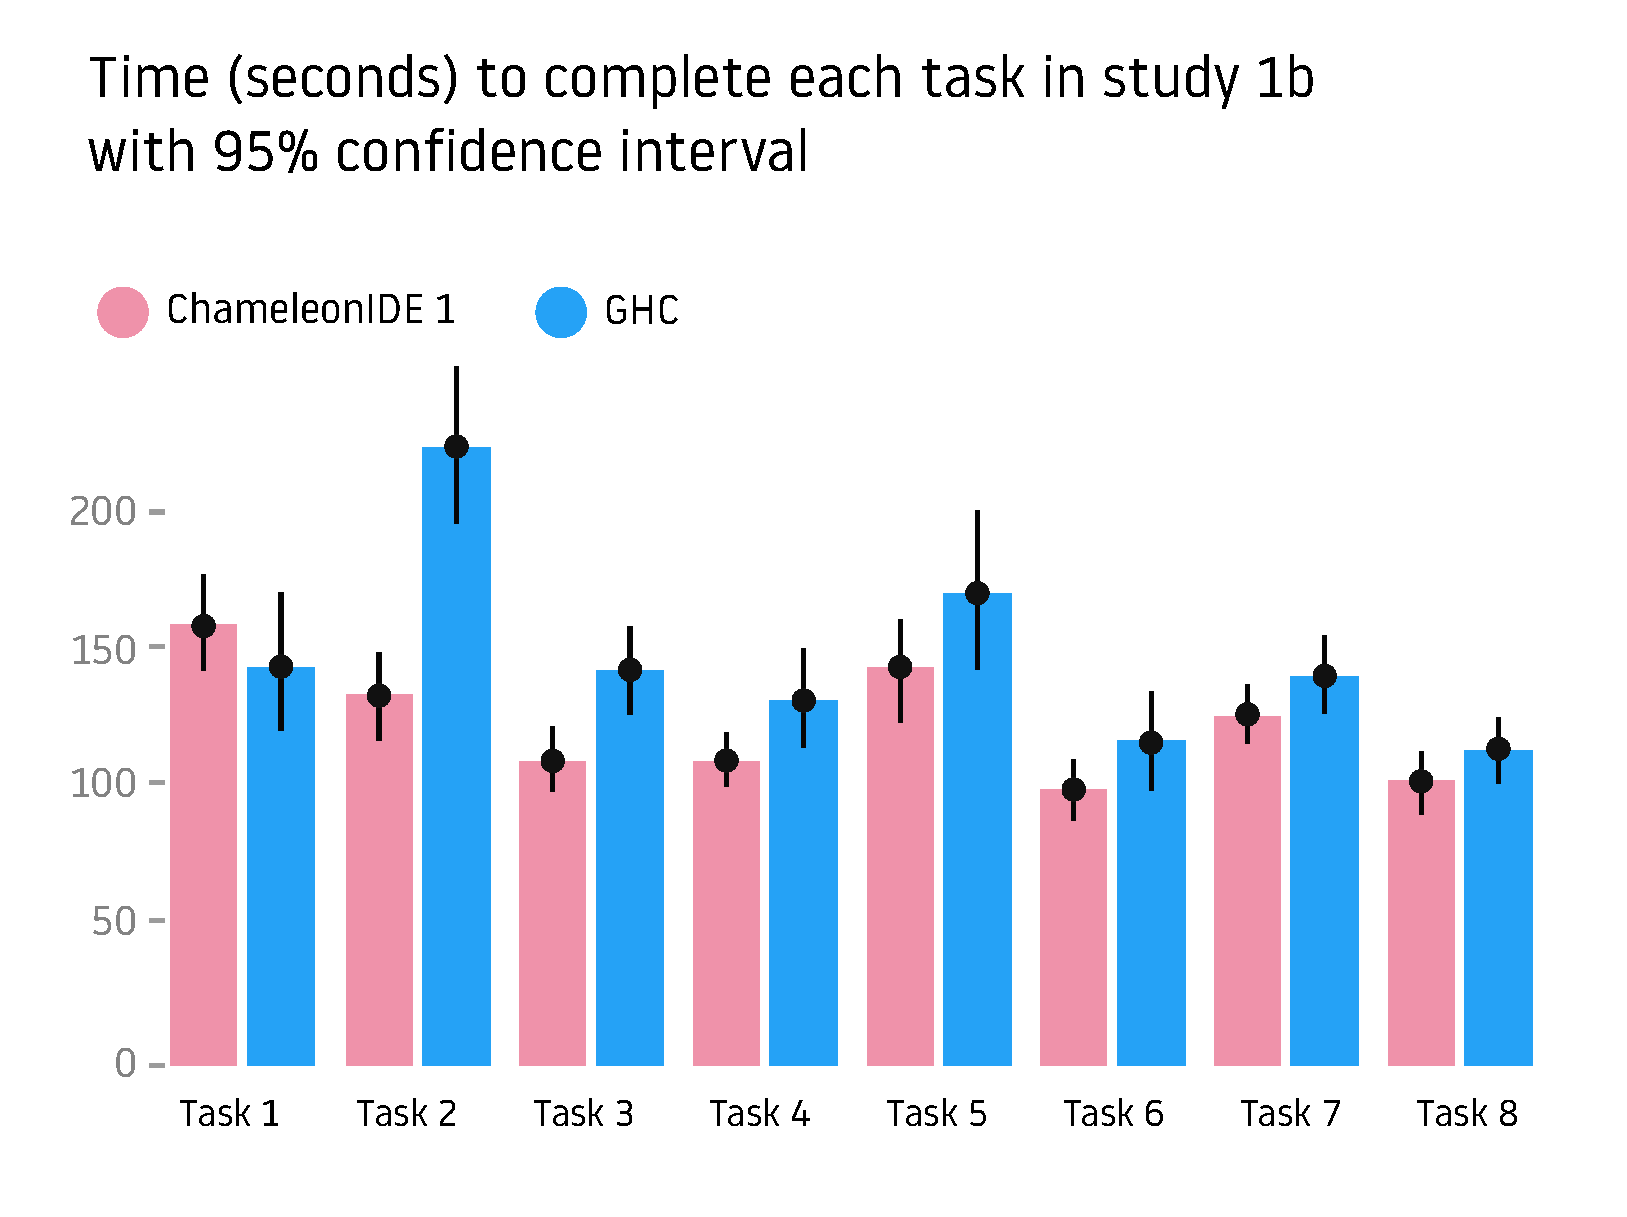
\includegraphics[width=0.8\linewidth,trim=12mm 15mm 12mm 35mm,clip]{images/user-study-1b.pdf}
    \caption{Study 1b task completion time (secs.) with 95\% confidence interval.}
    \label{fig:analysis-1b}
\end{figure}

\subsubsection*{\textbf {Results}}

The data collected during study 1a, Fig.~\ref{fig:analysis-1a} does not show significant differences across Tasks 1-7. In hindsight, these tasks were trivial challenges for most users, and the individual differences among participants are generally more significant than the differences between treatments. However, one interesting observation is task 8, where the \chameleon{} group outperformed the GHC group. We attribute this significant difference to the difficulty of Task 8. The source file is longer and involves more language features (abstract data types and high-level functions). GHC struggles to produce a relevant error message for this type of error. 
From this result, we hypothesized that we might observe a more significant difference using tasks with lengthier and more realistic source code. 
This hypothesis is also supported by the most common feedback claiming that the tasks were too trivial to invite meaningful evaluation. One participant said, ``Looks nicer than GHC, but without trying it on something more complicated, I cannot conclude whether it would help me in practice." 

Therefore, in study 1b we introduced more difficult challenges and indeed observed that the \chameleon{} group was faster than the GHC group in almost all tasks (figure \ref{fig:analysis-1b}), barring task 1. A two-sample paired t-test was performed to compare the completion time between \chameleon{} and GHC groups. There was a significant difference between the two groups: $t(23) = -3.86, p = 0007$. For task 1, it is suspected that some participants spent more time exploring the interface of \chameleon{} due to its unfamiliarity. For all other tasks, from the video recordings, we saw many \chameleon{} users confidently skip reading unrelated chunks of code, while GHC users generally read through the whole program. In harder problems and messier code, we notice programmers start to report the benefits of \chameleon{}. ``It's most useful feature that I noticed was that it points out the locations of both conflicting uses; GHC often makes it difficult to figure out how it's coming to a conclusion about a type." reported one participant. ``I think \chameleon{}  does a much better job than GHC's error messages. I like that it shows the sources for the type judgments. This makes it quite easy to figure out how to rectify errors." reported another participant.

% \begin{itemize}
%     \item {It has a longer source file than other tasks (only shorter than task 6, but task
%     6 contains two independent type errors while task 8 is one connected task
%     error);}
%     \item {It is more complex than others (involves abstract data types and function application); and
%     }
%     \item {
%         GHC struggles to produce a relevant error message for this type of error.
%     }
%   \end{itemize}


  

% \begin{figure}[H]
%     \centering
%     \Description{A screenshot from user study 1}
%     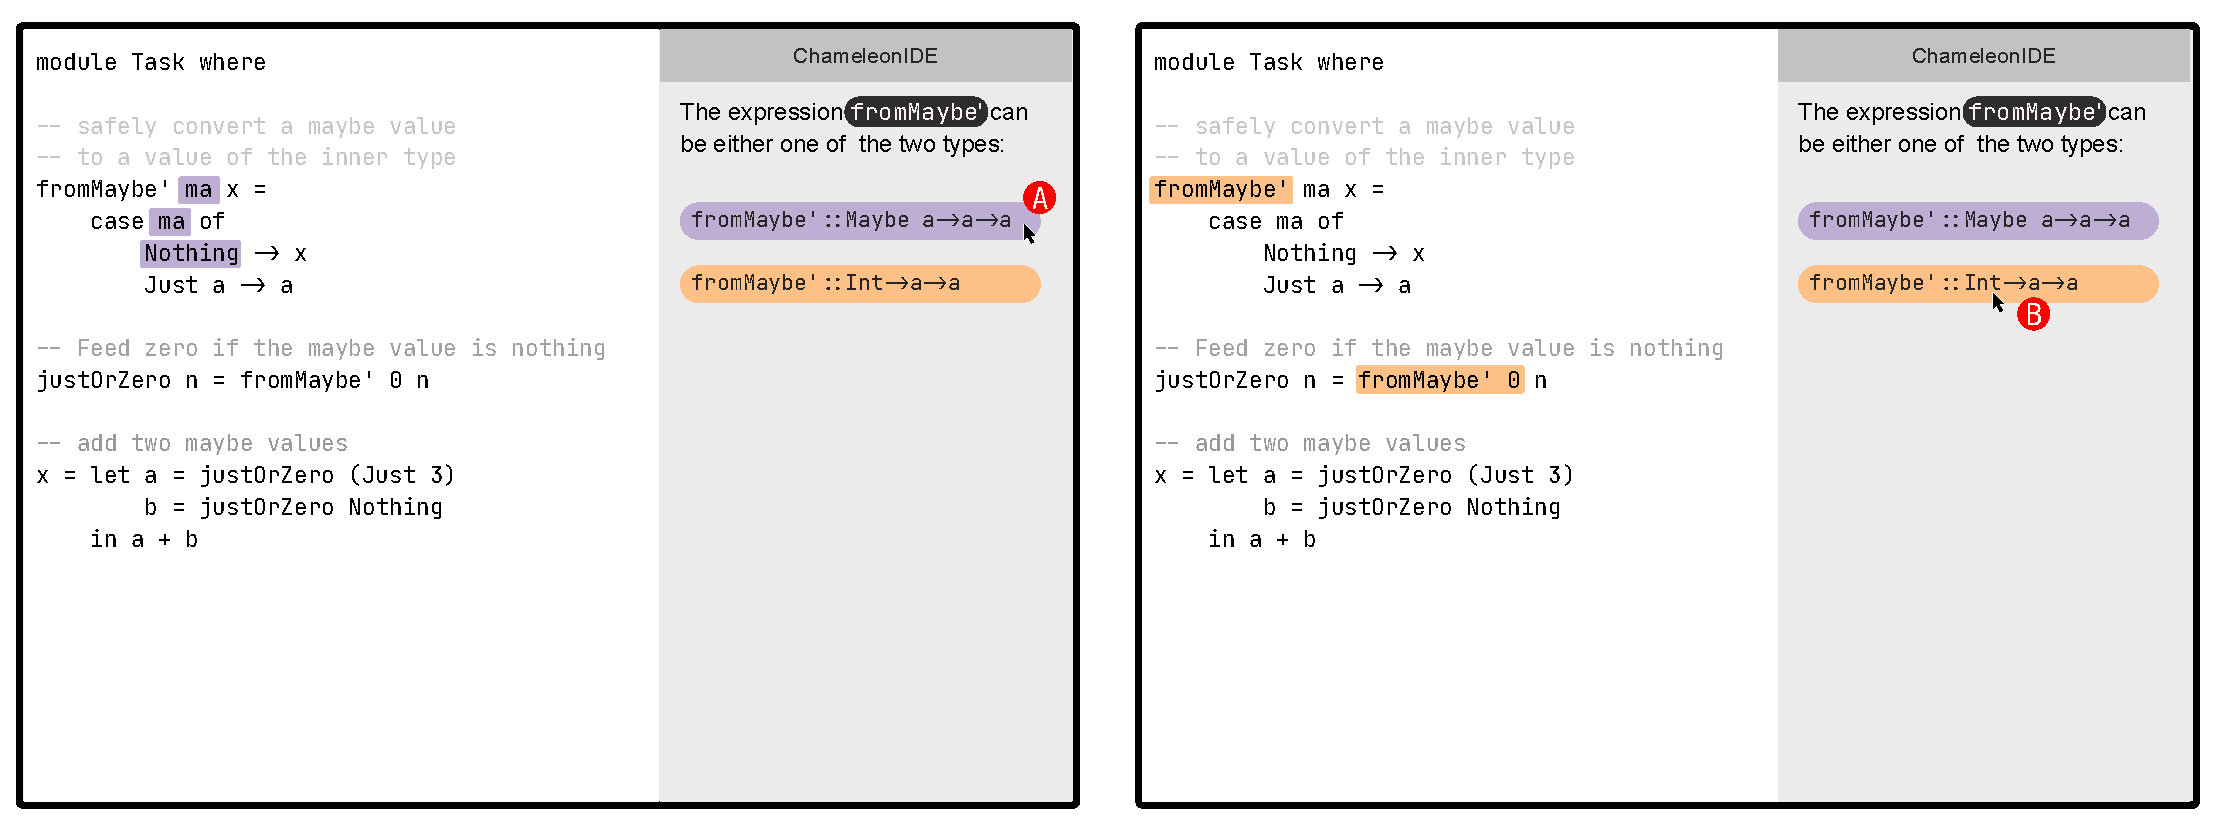
\includegraphics[width=\textwidth]{round1-screenshot.pdf}
%     \caption{
% One participant working with \chameleon{}  managed to identify the most probable location of the error (the application of `fromMaybe'` on line 11) by hovering over the two alternative types. The participant then quickly realized that the first argument `0` (highlighted in orange) is inconsistent with the definition where it is case matched to a `Nothing` value (highlighted in purple). After two retries with short hesitation the participant found the correct fix (by reversing the order of `0` and `n`).
%     }
%     \label{fig:r1-task8}
% \end{figure}


% \begin{figure}[htb]
%     \centering
%     \Description{A screenshot from user study 1}
%     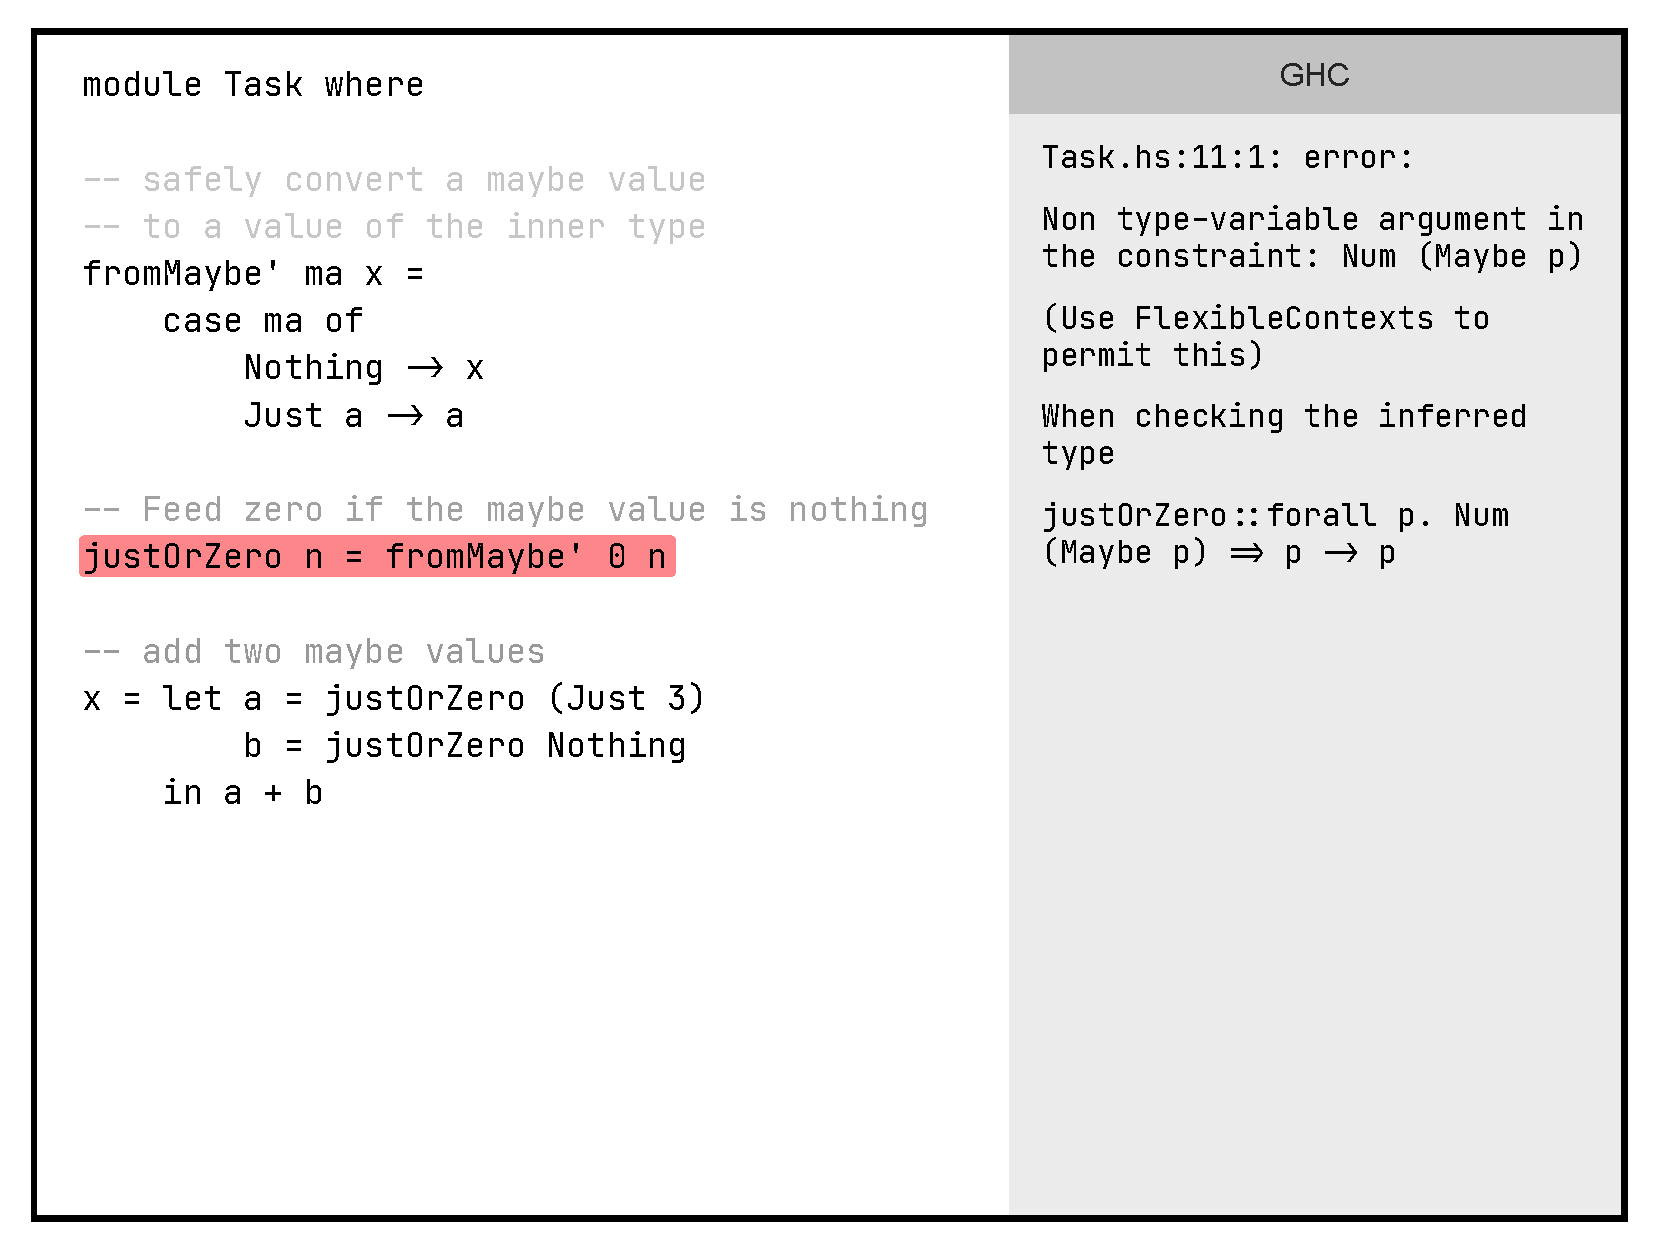
\includegraphics[width=\textwidth]{round1-screenshot-ghc.pdf}
%     \caption{
%         In task 8, participants using GHC took longer pauses at this task before committing to further investigation, either carefully reading the whole text or figuring out the meaning of the error message. The GHC error message is unfortunately unhelpful for this task.
%     }
%     \label{fig:task8-ghc}
% \end{figure}




\subsubsection{\textbf{\chameleon{} 2}}  \label{sub:us4}
Based on observations of Study 1 we introduced several new features to \chameleon{}, eventually resulting in the UI depicted in Figs.~(2-13). Interactive features were available in this iteration, such as deduction steps, candidate expressions, and mode switching. A few other user interfaces \cite{Fu2021-xd} were designed and prototyped between the development of \chameleon{} 1 and \chameleon{} 2. Study 2 addresses the research question: 

\noindent\textbf{RQ2:} \textit{How do programmers use the interactive features in \chameleon{} 2?}. 

More specifically:
\begin{itemize}
    \item \textbf{RQ2.1} How do programmers use the advanced features provided by \chameleon{} 2?
    \item \textbf{RQ2.2} Do programmers prefer switching modes during debugging type errors?
    \item  \textbf{RQ2.3} What are programmers' preferences among the three modes provided by \chameleon{} 2?


\end{itemize}

During each run, the initial mode of each task alternated through the three different modes and repeated three cycles in nine tasks. The order of the three modes in each cycle is counterbalanced among all participants. However, participants can switch to other modes at any time. 



% \begin{figure}[h]
%     \centering
%     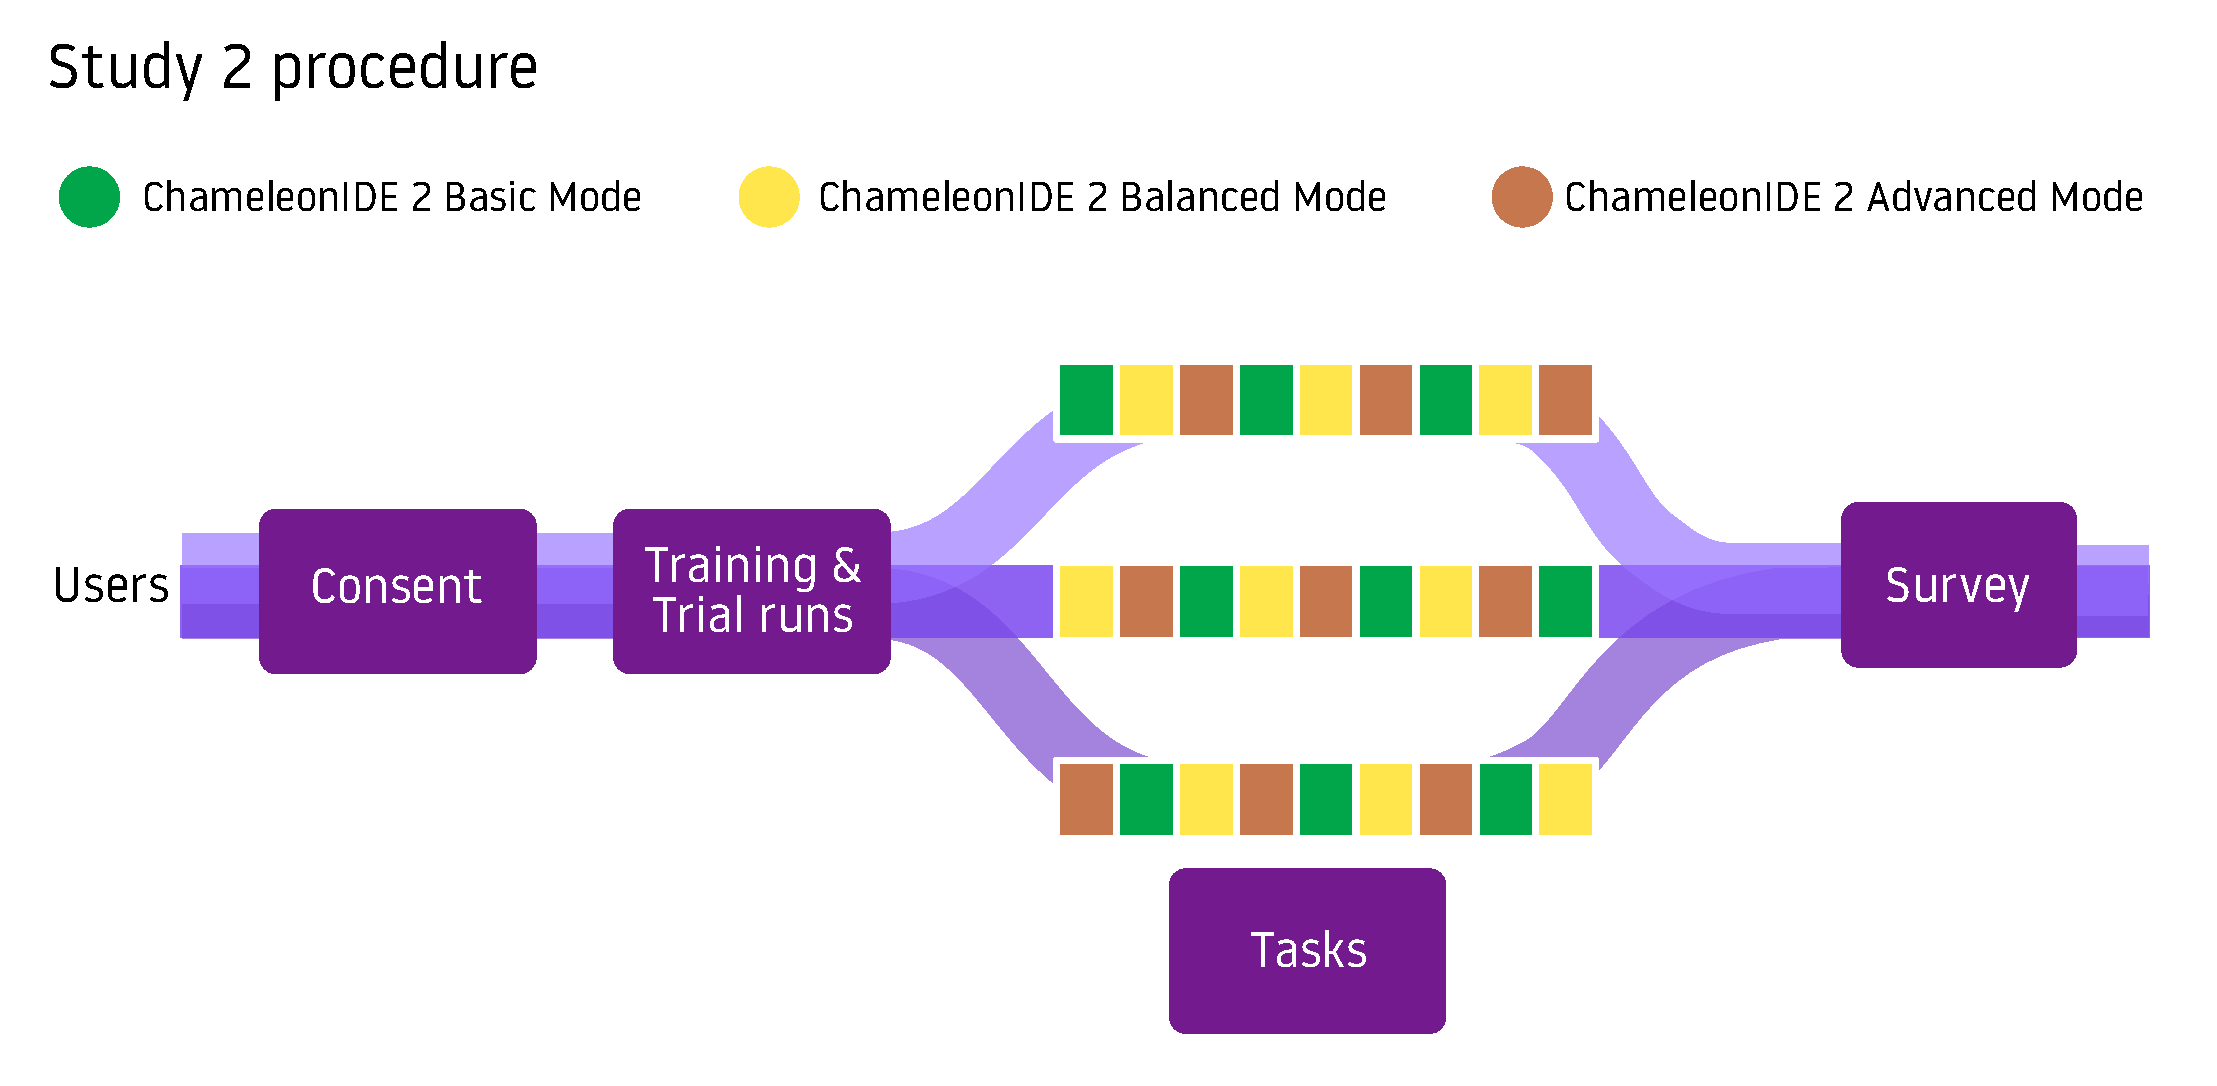
\includegraphics[width=\linewidth]{images/procedure-2.pdf}
%     \caption{\todo{Does this figure really help at all?}}
%     \label{fig:procedure-2}
% \end{figure}

\subsubsection*{\textbf{Results}} 

Study 2 is more exploratory in methodology than Study 1. We encouraged programmers  to discover their way of using the tool. In post hoc analysis of the collected log data, we were able to extrapolate some interesting patterns of how the tool was used. 


\textbf{RQ2.1}. The most striking feature of the data is that users tend to vary wildly in their use of the tool. Some users used the features extensively, while others completed the tasks without actively exploring the given information. Based on this discrepancy, we divided the users into three groups in table~\ref{tab:interaction-level}.
\begin{table}
    \centering
\begin{scriptsize}
\begin{small}
\noindent\begin{tabularx}{\linewidth}{ 
  | >{\hsize=.26\hsize}X 
  | >{\hsize=.74\hsize \raggedright\arraybackslash}X  | }
    \hline
        Interaction level & Description \\ \hline
        \textit{Minimal}  & Users completed the tasks by making changes in source code, type checking, and reading error messages. \\ \hline
        \textit{Low}  & Users only actively used universal features in all modes, for example, hovering on "Possible type 1" and "Possible type 2" to narrow down error space. \\ \hline
        \textit{High}  & Users did everything from the low interaction group but used features specific to the Balanced mode and the Advanced mode, such as activating steps and expression cards. \\ \hline
\end{tabularx}
\end{small}
\end{scriptsize}
    \caption{Levels of programmer interaction and their description}
    \label {tab:interaction-level}
\end{table}

As shown in  Fig.~\ref{fig:r4-analysis}, the time to complete each task roughly relates to the interaction level of participants. Participants with higher interaction levels generally performed better, and the lowest interaction level was worse. Tukey’s HSD Test for multiple comparisons found that the completion time was significantly different between the minimal interaction group and the high interaction group ($p \le 0.001$, 95\% C.I. = [18.26, 31.41]), and between the minimal interaction group and the low interaction group ($p \le 0.001$, 95\% C.I. = [11.96, 26.67]). The results from three tasks stand out from the general trend: in Tasks 4 and 6, higher interaction users performed worse, and in task 9, the general trend is exaggerated. As with Study 1a and 1b, this difference is likely related to task difficulty. Tasks 4 and 6 are shorter than other tasks. The ideal fixes for these two tasks are placed relatively early in the source code (both in the first two lines of the source code). Users simply reading top to bottom could quickly identify the error without needing to skip unrelated sections of code using the information provided by \chameleon{}. This reduced the apparent benefit of \chameleon{} in these tasks. On the other hand, task 9 is the lengthiest task of all. It also involves deeply nested type definitions that are harder to follow in mind.

\begin{figure}
    \centering
    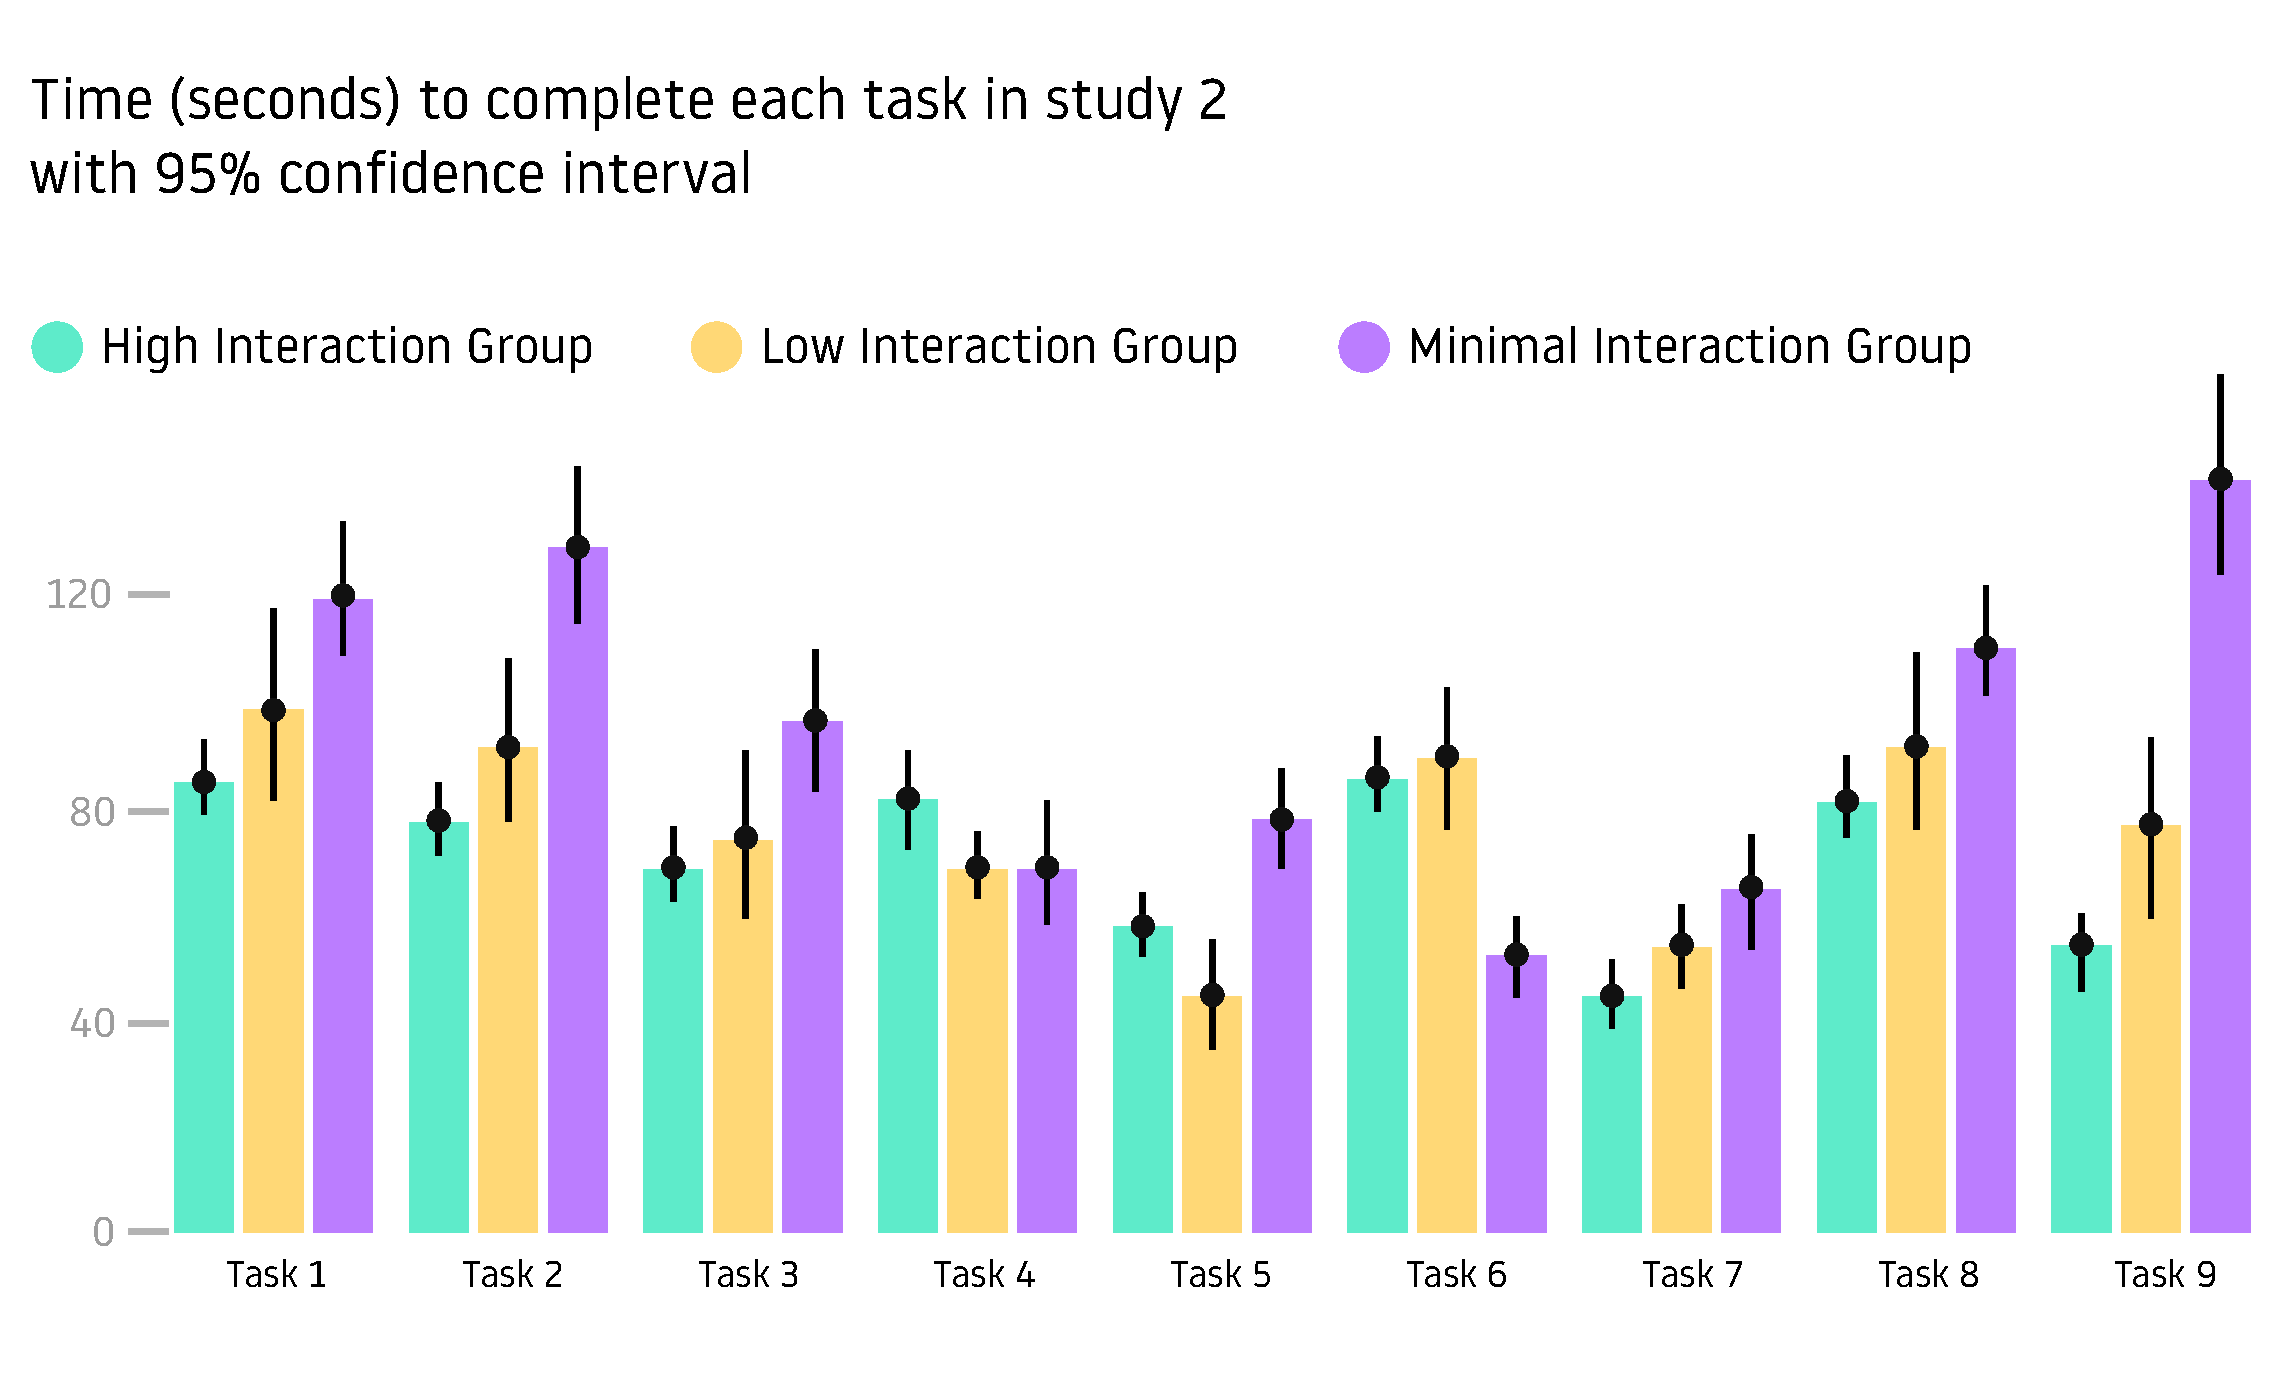
\includegraphics[width=\linewidth,trim=0mm 15mm 0mm 50mm,clip]{images/user-study-2.pdf}
    \caption{Study 2 task completion time (secs.) with 95\% confidence intervals.}
    \label{fig:r4-analysis}
\end{figure}


% \begin{figure}[h]
%     \centering
%     \includegraphics[width=\linewidth]{images/r4-task9.png}
%     \caption{
% High interaction users were able to locate the exact line for a potential fix after navigating to deduction step 6 or 7, which directly revealed the true cause of the type error. After this, 12 out of 15 high interaction users provided the most ideal fix in the first try. Low interaction group  takes longer time to examine the problem, provided wrong fixes in the initial trials. One participant fixed a minor run-time issue (a problematic pattern matching of `[attributes]` on line 18) however failed to identify the culprit of the type error. This location is not pinpointed by \chameleon{} and therefore it is understandable that programmers who used the deduction steps would be able to ignore this part of the source code.
%     }
%     \label{fig:r4-task9}
% \end{figure}


Another observation is when using the mode switching feature of \chameleon{}, we show this by presenting the starting mode and finishing mode of each task and each participant in a correlation matrix (Fig. \ref{fig:r4-mode-switching}). This observation suggests two characteristics of using multi-mode debugging tools. First, to answer \textbf{RQ2.2} programmers are roughly splitted in this matter: 53\% changing modes vs. 47\% staying in the same mode. Second, to answer \textbf{RQ2.3} when changing modes, programmers generally switch to the more informative modes instead of the more concise ones.
\begin{figure}
    \centering
    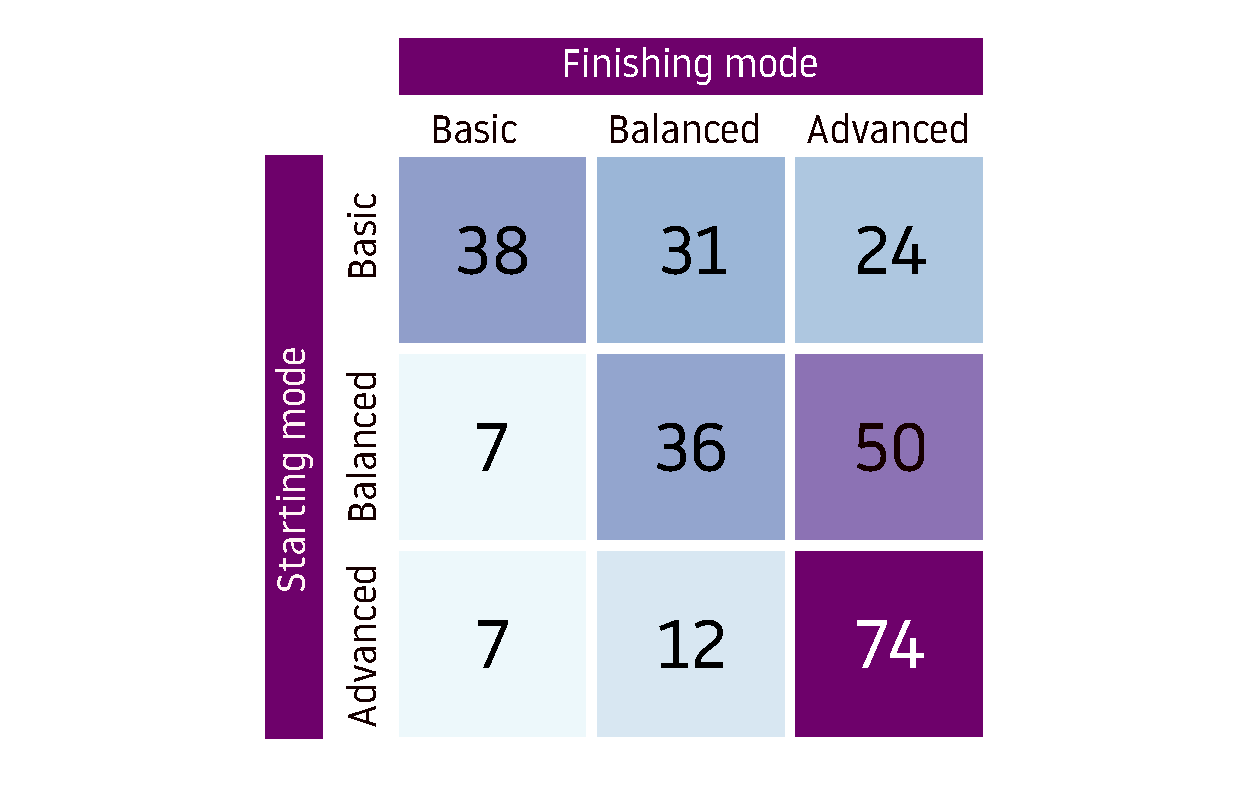
\includegraphics[width=0.7\linewidth,trim=0mm 5mm 0mm 5mm,clip]{images/mode-switching.pdf}
    \caption{Study 2 mode switches by starting mode.  Users overwhelmingly switched to the more sophisticated interface mode.
        % The rows represent the finishing mode, columns starting modes.
    }
    \label{fig:r4-mode-switching}
\end{figure}


\subsection{Limitations}

One threat to the validity of the evaluation is the number of participants. Although for each study we received hundreds of online participants, the studies suffered from a high abandonment rate (especially study 1b). This was expected: the programming challenges are difficult, and our volunteer participants are unremunerated. 
Because we recruited participants online and anonymized all the participants, it is possible for participants of a previous study to enter a later one. This creates variation in familiarity. We offset this by using new code challenges in every study and conducting trial runs before data collection to bring new participants up to speed.
Conducting studies remotely and unsupervised left us no means to intervene when users encounter usability issues. To mitigate this, we conducted cognitive walkthroughs and sandbox pilots before running each study.

Future evaluation would benefit from using more realistic tasks. The tasks in our human studies do not get as complex as professional Haskell programmers may face in a typical production codebase. It would be interesting to see how \chameleon{} is used against type errors that span multiple files and packages and include more confusing abstractions, like Monads, Monad transformers, and Lenses.
